\documentclass[10pt,a4paper]{article}
\usepackage[margin=1.7cm]{geometry}
\usepackage[T1]{fontenc}
\usepackage{lmodern}
\usepackage{xcolor}
\usepackage{booktabs}
\usepackage{array}
\usepackage{amsmath}
\usepackage{amssymb}
\usepackage{enumitem}
\usepackage{tabularx}
\usepackage{mdframed}
\usepackage{tikz}
\usetikzlibrary{positioning,arrows.meta,fit,backgrounds}
\usepackage{listings}
\usepackage[colorlinks=true]{hyperref}

% ── Palette (shared with the rest of docs/) ───────────────────────────────────
\definecolor{hdrblue}{RGB}{10,60,140}
\definecolor{accentteal}{RGB}{0,120,120}
\definecolor{okgreen}{RGB}{20,110,40}
\definecolor{badred}{RGB}{180,20,20}
\definecolor{warnamber}{RGB}{180,90,0}
\definecolor{newbg}{RGB}{210,235,255}
\definecolor{newtext}{RGB}{0,60,130}
\definecolor{rulegray}{RGB}{130,130,130}
\definecolor{tablegray}{RGB}{245,246,248}
\definecolor{codebg}{RGB}{246,248,250}
\definecolor{stepfill}{RGB}{222,236,255}
\definecolor{warnbg}{RGB}{255,243,224}
\definecolor{okbg}{RGB}{223,244,228}

\hypersetup{linkcolor=hdrblue, urlcolor=accentteal,
  pdftitle={FPGA Tick-to-Trade: SDF Timing Simulation Guide}}

\setlength{\parindent}{0pt}
\setlength{\parskip}{4pt}

\newcommand{\sectionrule}{\par\nobreak\vspace{1pt}\textcolor{rulegray}{\rule{\linewidth}{0.8pt}}\par\vspace{1pt}}
\newcommand{\fpath}[1]{\texttt{\textcolor{hdrblue}{#1}}}

\lstdefinestyle{sh}{
  basicstyle=\ttfamily\footnotesize, backgroundcolor=\color{codebg},
  frame=single, framerule=0pt, rulecolor=\color{rulegray},
  breaklines=true, columns=fullflexible, keepspaces=true,
  xleftmargin=4pt, xrightmargin=4pt, aboveskip=4pt, belowskip=4pt,
  literate={~}{{\textasciitilde}}1
}

\newmdenv[linecolor=newtext, backgroundcolor=newbg, linewidth=1.2pt,
  leftmargin=0pt, rightmargin=0pt, innerleftmargin=8pt, innerrightmargin=8pt,
  innertopmargin=6pt, innerbottommargin=6pt, skipabove=6pt, skipbelow=6pt]{keybox}
\newmdenv[linecolor=badred, backgroundcolor=warnbg, linewidth=1.2pt,
  leftmargin=0pt, rightmargin=0pt, innerleftmargin=8pt, innerrightmargin=8pt,
  innertopmargin=6pt, innerbottommargin=6pt, skipabove=6pt, skipbelow=6pt]{warnboxx}
\newmdenv[linecolor=okgreen, backgroundcolor=okbg, linewidth=1.2pt,
  leftmargin=0pt, rightmargin=0pt, innerleftmargin=8pt, innerrightmargin=8pt,
  innertopmargin=6pt, innerbottommargin=6pt, skipabove=6pt, skipbelow=6pt]{okboxx}

\tikzset{
  flowstep/.style ={rectangle, rounded corners=2pt, draw=hdrblue, fill=stepfill,
                text width=2.7cm, align=center, font=\footnotesize, minimum height=1.0cm, thick},
  flow/.style ={-{Stealth[length=2.2mm]}, thick, draw=hdrblue},
}

\begin{document}

{\LARGE\bfseries\color{hdrblue} SDF Timing Simulation \textendash{} How-To Guide}%
\hfill{\small\color{rulegray} 17 June 2026}\\[-2pt]
{\large\color{accentteal} Running the implemented FPGA design with real silicon delays \textendash{} no chip needed}

\textcolor{hdrblue}{\rule{\linewidth}{2pt}}

\begin{keybox}
{\large\bfseries\color{newtext} What this is, in one paragraph}

\smallskip
A normal RTL simulation assumes \emph{zero} gate and wire delay --- it only checks
logic, cycle by cycle. A \textbf{post-implementation timing simulation} replays the
\emph{actual placed-and-routed} design with the \emph{real} propagation delay of
every gate and every wire, supplied by an \textbf{SDF} file (Standard Delay
Format). It is the most silicon-accurate behavioural check you can run
\emph{without a physical FPGA}. This guide documents exactly how we generated and
ran it for \fpath{tick\_to\_trade\_top}, including the traps that cost time, so it
can be repeated.
\end{keybox}

% ── What is SDF ───────────────────────────────────────────────────────────────
{\large\bfseries\color{hdrblue} 1.\quad What is SDF, and why use it?}
\sectionrule

\textbf{SDF (Standard Delay Format)} is a text file Vivado writes \emph{after}
place-and-route. For every cell instance it lists the real timing: input-to-output
propagation delays (\texttt{IOPATH}), setup/hold requirements (\texttt{SETUP},
\texttt{HOLD}), pulse widths, etc. --- all extracted from the routed design for the
target device (here \texttt{xcu200}, Virtex UltraScale+).

\textbf{Back-annotation} is the act of loading those delays onto a gate-level
netlist during simulation, so each signal transition arrives \emph{late} by its
true physical delay instead of instantly. Three things it buys you:

\begin{itemize}[leftmargin=1.4em, topsep=2pt, itemsep=1pt]
\item Confirms the design still behaves correctly when signals have real delays.
\item Surfaces any setup/hold timing violation \emph{dynamically} (as an X or
      glitch) --- a cross-check on the static timing analysis.
\item Gives a delay-accurate view of the tick-to-trade path at the 5\,ns
      (200\,MHz) clock.
\end{itemize}

\begin{keybox}
\textbf{Relationship to static timing (STA).} Vivado's STA already proved the
design closes timing (WNS\,$>$\,0 at 200\,MHz) by analysing every path's delay
mathematically. A \emph{passing} SDF simulation is the dynamic confirmation of the
same fact. STA is the proof; the SDF sim is the live demonstration.
\end{keybox}

% ── Prerequisites ─────────────────────────────────────────────────────────────
{\large\bfseries\color{hdrblue} 2.\quad Prerequisites (what you need locally)}
\sectionrule

\begin{center}\small
\renewcommand{\arraystretch}{1.2}
\begin{tabularx}{\linewidth}{@{}>{\raggedright\arraybackslash}p{4.6cm} X@{}}
\toprule
\textbf{Need} & \textbf{Here} \\
\midrule
Vivado (synth/impl + write SDF) & \fpath{\textasciitilde/Xilinx/2025.2/Vivado}; \texttt{source \textasciitilde/Xilinx/2025.2/Vivado/settings64.sh} \\
A simulator                     & \textbf{xsim} (ships inside Vivado, with \emph{precompiled} libraries --- no \texttt{compile\_simlib} needed). QuestaSim also works but needs the libs compiled first. \\
A synthesis checkpoint          & \fpath{Vivado/HFT/HFT.srcs/utils\_1/imports/synth\_1/tick\_to\_trade\_top.dcp} \\
A physical FPGA                 & \textbf{Not required.} This is pure simulation. \\
\bottomrule
\end{tabularx}
\end{center}

% ── The flow ──────────────────────────────────────────────────────────────────
{\large\bfseries\color{hdrblue} 3.\quad The Flow at a Glance}
\sectionrule

\begin{center}
\resizebox{\linewidth}{!}{%
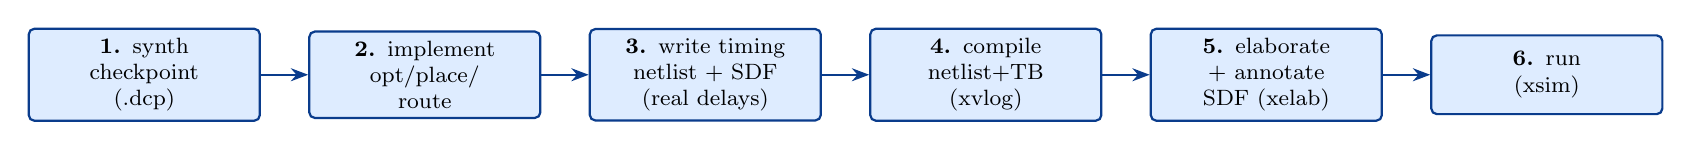
\begin{tikzpicture}[node distance=6mm]
\node[flowstep] (a) {\textbf{1.} synth\\ checkpoint\\ (.dcp)};
\node[flowstep, right=of a] (b) {\textbf{2.} implement\\ opt/place/\\ route};
\node[flowstep, right=of b] (c) {\textbf{3.} write timing\\ netlist + SDF\\ (real delays)};
\node[flowstep, right=of c] (d) {\textbf{4.} compile\\ netlist+TB\\ (xvlog)};
\node[flowstep, right=of d] (e) {\textbf{5.} elaborate\\ + annotate\\ SDF (xelab)};
\node[flowstep, right=of e] (f) {\textbf{6.} run\\ (xsim)};
\foreach \x/\y in {a/b,b/c,c/d,d/e,e/f} \draw[flow] (\x) -- (\y);
\end{tikzpicture}}
\end{center}

Steps 1--3 are Vivado (\fpath{gatesim/impl\_and\_timesim.tcl}); steps 4--6 are xsim
(\fpath{gatesim/run\_timesim\_xsim.sh}). All artifacts live in \fpath{gatesim/}.

% ── Step detail ───────────────────────────────────────────────────────────────
{\large\bfseries\color{hdrblue} 4.\quad Steps 1\textendash3: Implement \& Write the SDF (Vivado)}
\sectionrule

Script \fpath{gatesim/impl\_and\_timesim.tcl} opens the synthesis checkpoint,
implements it, then emits the timing netlist and the SDF:

\begin{lstlisting}[style=sh]
open_checkpoint .../synth_1/tick_to_trade_top.dcp
opt_design; place_design; phys_opt_design; route_design
write_checkpoint -force gatesim/tick_to_trade_top_routed.dcp

# the two timing-sim artifacts:
write_sdf     -force gatesim/tick_to_trade_top_time.sdf
write_verilog -force -mode timesim -sdf_anno true \
              -sdf_file gatesim/tick_to_trade_top_time.sdf \
              gatesim/tick_to_trade_top_timesim.v
\end{lstlisting}

Run it:
\begin{lstlisting}[style=sh]
source ~/Xilinx/2025.2/Vivado/settings64.sh
vivado -mode batch -source gatesim/impl_and_timesim.tcl
\end{lstlisting}

\textbf{What you get:} \fpath{tick\_to\_trade\_top\_timesim.v} (the gate netlist,
$\approx$8{,}000 cells: LUTs/FFs/CARRY8/RAMB) and
\fpath{tick\_to\_trade\_top\_time.sdf} ($\approx$18\,MB of delays). Crucially,
\texttt{-sdf\_anno true} \textbf{embeds} a \texttt{\$sdf\_annotate("...sdf")} call
\emph{inside} the netlist, so the simulator loads the SDF automatically --- you do
\emph{not} pass the SDF again on the command line.

% ── Step detail xsim ──────────────────────────────────────────────────────────
{\large\bfseries\color{hdrblue} 5.\quad Steps 4\textendash6: Compile, Annotate, Run (xsim)}
\sectionrule

Script \fpath{gatesim/run\_timesim\_xsim.sh}:

\begin{lstlisting}[style=sh]
# 4) compile netlist + testbench + glbl (Xilinx global-reset module)
xvlog -sv tick_to_trade_top_timesim.v
xvlog -sv tb_timesim.sv
xvlog ~/Xilinx/2025.2/data/verilog/src/glbl.v

# 5) elaborate -- LIBRARY ORDER IS CRITICAL (see traps below)
xelab -timescale 1ps/1ps \
      -L simprims_ver -L secureip -L unisims_ver \
      tb_timesim glbl -s tb_snapshot -log xelab_run.log

# 6) run
xsim tb_snapshot -runall -log xsim_run.log
\end{lstlisting}

The testbench \fpath{gatesim/tb\_timesim.sv} drives the BUY scenario (an ask then a
bid that makes the book bid-heavy), waits for the decision on \texttt{m\_axis}, and
reads the hardware latency counter over AXI-Lite. The exact ITCH message bytes were
dumped from the Python encoder (\fpath{sim/synth\_itch.py}) and hard-coded so they
are byte-accurate.

\begin{okboxx}
\textbf{Success looks like this in the log:}
\begin{lstlisting}[style=sh]
[XSIM 43-3451] SDF backannotation process started ... root module "tb_timesim/dut".
[XSIM 43-3452] SDF backannotation was successful ...
\end{lstlisting}
That second line is the goal: the real delays are now applied. The design then
simulated at 200\,MHz with \textbf{no timing-violation failure}, consistent with
the static-timing closure (WNS\,$>$\,0).
\end{okboxx}

% ── Traps ─────────────────────────────────────────────────────────────────────
{\large\bfseries\color{hdrblue} 6.\quad The Traps (these cost real time)}
\sectionrule

\begin{warnboxx}
\textbf{Trap 1 \textendash{} Library order (the big one).}
An \emph{implemented} netlist instantiates \textbf{SIMPRIM} primitives
(\texttt{IBUFCTRL}, \texttt{INBUF}, \texttt{RAMD64E}). In \texttt{xelab} the
\texttt{-L} libraries are searched \emph{in order}, so \texttt{simprims\_ver} and
\texttt{secureip} \textbf{must be listed before} \texttt{unisims\_ver}. Get it
wrong and the cells bind to the \emph{functional} unisim models, which abort with:
\begin{lstlisting}[style=sh]
Error: [Unisim IBUFCTRL-103] SIMPRIM primitive is not intended for direct
instantiation in RTL or functional netlists ...
\end{lstlisting}
The \emph{same} wrong order also makes SDF annotation fail with
\texttt{[XSIM 43-3462] Unable to annotate SDF delays}. Fixing the order fixed both.
Correct: \texttt{-L simprims\_ver -L secureip -L unisims\_ver}.
\end{warnboxx}

\begin{warnboxx}
\textbf{Trap 2 \textendash{} Do not annotate the SDF twice.}
Because \texttt{write\_verilog -sdf\_anno true} \emph{embeds} \texttt{\$sdf\_annotate}
in the netlist, do \textbf{not} also pass \texttt{-sdfmax} to \texttt{xelab} ---
the two conflict and annotation fails. Rely on the embedded call only.
\end{warnboxx}

\begin{warnboxx}
\textbf{Trap 3 \textendash{} QuestaSim only (if you skip xsim).}
\texttt{compile\_simlib} for QuestaSim broke on two things: (a) the install path
has a \emph{space} (\fpath{/home/abhishek/QuestaSim 2021.2.1/...}) which breaks
\texttt{execve} --- fix with a no-space symlink; (b) \texttt{-library} only accepts
\texttt{unisim}, \texttt{simprim}, or \texttt{all}, and \texttt{all} compiles
\emph{every} IP (30+ min). \textbf{Easiest path: use xsim}, whose libraries are
already precompiled --- no \texttt{compile\_simlib} at all.
\end{warnboxx}

\begin{warnboxx}
\textbf{Trap 4 \textendash{} Gate-level RAM starts as X.}
In gate-level simulation the order-book memories (\texttt{RAMD64E},
\texttt{RAMB36E2}) power up to \texttt{X} (RTL sim quietly defaults them to 0). With
the book uninitialised, a minimal 2-message scenario may not produce a clean
decision. This is a \emph{simulation-init} nuance, \textbf{not} a hardware bug ---
decision correctness is already proven by the 95/95 RTL tests and the
software-equivalence shadow test. To also capture a decision in gate sim you would
initialise the memories or warm the book with more traffic. Two testbench details
that matter regardless: drive the AXI-Stream master so each byte is \emph{held
until} \texttt{tready} accepts it, and hold reset long enough ($\approx$30 cycles)
to clear the Xilinx global set/reset (\texttt{glbl.GSR}, $\approx$100\,ns).
\end{warnboxx}

% ── Re-run ────────────────────────────────────────────────────────────────────
{\large\bfseries\color{hdrblue} 7.\quad How to Re-run It (quick reference)}
\sectionrule

\begin{lstlisting}[style=sh]
cd ~/Projects/HFT
source ~/Xilinx/2025.2/Vivado/settings64.sh

# (1-3) implement + write timing netlist & SDF  [~3 min]
vivado -mode batch -source gatesim/impl_and_timesim.tcl

# (4-6) compile, SDF-annotate, run in xsim       [xelab ~10 min w/ SDF]
bash gatesim/run_timesim_xsim.sh

# look for: "[XSIM 43-3452] SDF backannotation was successful"
grep -i "backannotation" gatesim/xelab_run.log
\end{lstlisting}

\begin{center}\small
\renewcommand{\arraystretch}{1.2}
\begin{tabularx}{\linewidth}{@{}>{\raggedright\arraybackslash}p{6.0cm} X@{}}
\toprule
\textbf{File (\fpath{gatesim/})} & \textbf{Role} \\
\midrule
\fpath{impl\_and\_timesim.tcl}            & Vivado: implement + write netlist + SDF \\
\fpath{tick\_to\_trade\_top\_timesim.v}   & gate netlist (with embedded \$sdf\_annotate) \\
\fpath{tick\_to\_trade\_top\_time.sdf}    & the real cell + routing delays ($\approx$18\,MB) \\
\fpath{tick\_to\_trade\_top\_routed.dcp}  & implemented checkpoint (reuse without re-routing) \\
\fpath{tb\_timesim.sv}                    & timing testbench (drives BUY scenario) \\
\fpath{run\_timesim\_xsim.sh}             & xsim compile + SDF-annotate + run \\
\bottomrule
\end{tabularx}
\end{center}

\vfill
{\small\color{rulegray} Companion: \fpath{hardware\_in\_the\_loop.pdf} (what runs a
live trade vs.\ what is verified), \fpath{implementation\_results.pdf} (STA timing /
area / power). Build: \texttt{pdflatex sdf\_timing\_sim\_guide.tex}.}

\end{document}
